\chapter{Extending Bigram Grammars}
\label{cha:SLMath}

Bigram grammars are a step in the right direction from the initial list phonology model.
Every grammar is still just a list of items, but now we use this list to determine the well-formedness of a word in a compositional manner.
The problem of bigram grammars is that they are not powerful enough to capture certain phonological processes like intervocalic voicing --- in linguistic parlance, the size of the grammars' locality domain is limited to two adjacent symbols, so bigger contexts cannot be represented correctly.
The obvious solution is to extend the size of the scanner window so that the grammar uses trigrams, 4-grams, or maybe even something bigger.
We will see today that this generalization is a natural one in the sense that it preserves the essential properties of bigram grammars while increasing their empirical coverage.

\section{Generalization to Strictly Local Grammars}

Lifting the notion of bigrams to arbitrary $k$-grams works almost exactly as one would suspect.
The set of trigrams of the string $\String{abcd}$, for example, includes $\String{\LeftEdge a b}$, $\String{abc}$, $\String{bcd}$, and $\String{cd\RightEdge}$.
However, it also includes $\String{\LeftEdge \LeftEdge a}$ and $\String{d \RightEdge \RightEdge}$.
Why the extra trigrams with multiple edge markers?
For one thing, we still want to directly express basic facts like ``a word may start with $a$'', while the trigram $\String{\LeftEdge a b}$ encodes ``a word may start with $a$ followed by $b$''.
More importantly, as the length of $k$-grams increase, more and more words won't have a single $k$-gram unless we pad them with $k-1$ edge markers.
For example, the augmented version of the empty string would just be $\LeftEdge \RightEdge$, which is too short for a trigram.
Similarly, the string $\String{ab}$ would be $\String{\LeftEdge ab \RightEdge}$, which is too short any $k$-gram with $k > 4$.
The simplest solution is to simply add $k-1$ edge markers instead of just a single one.
For bigrams, the number of edge markers does not change since $2 - 1 = 1$.

On the formal side, the generalization from bigrams to $k$-grams requires but a few minor modifications in our original definition.
We also use this opportunity to slightly change our terminology: instead of \emph{$k$-gram grammar} and \emph{$k$-gram languages}, we will speak of \emph{strictly $k$-local grammars} and \emph{strictly $k$-local languages}.
This will make it easier later on to distinguish this formalism from a related one that also operates with $k$-grams but interprets them differently.

\begin{definition}[$k$-grams]
    Let $k$ be some natural number.
    A \emph{$k$-gram}, or \emph{$k$-factor}, over alphabet $\Sigma$ is an element of $(\Sigma \cup \setof{\LeftEdge, \RightEdge})^k$.
    Given a string $w$ over $\Sigma$, its \emph{$k$-augmented} counterpart $\augmented{w}_k \is \LeftEdge^{k-1} \stringcat w \stringcat \RightEdge^{k-1}$ consists of $w$ with $k-1$ left edge markers and $k-1$ right edge markers, and its set of $k$-grams is given by
    \(
        \Bigrams[k](w) \is
            \setof{
                s \in (\Sigma \cup \setof{\LeftEdge, \RightEdge})^k
                \mid
                \exists u,v \in \Sigma^* \text{ s.t. }
                u \stringcat s \stringcat v = \augmented{w}
            }
    \).
\end{definition}
%
You can see that this definition of $k$-gram is a natural extension of the concept of bigrams for if we replace $k$ by $2$ in the definition, we get exactly the original definition of bigrams.
The concept of bigram languages is generalized in the same fashion to $k$-gram languages, which jointly form the class of \emph{strictly local languages}.
%
\Note{%
    Notice that the definition of strictly $k$-local also allows for $k = 0$.
    Can you list all strictly $0$-local languages?
    \emph{Hint}: There's only two of them.
}
%
\begin{definition}[Strictly Local Languages]
    A finite set of $k$-grams is called a \emph{strictly $k$-local grammar}.
    A positive strictly $k$-local grammar $G$ generates the language
    \(
        L(G) \is
            \setof{ w \mid \Bigrams[k](w) \subseteq G }
    \).
    A negative strictly $k$-local grammar $G$ generates the language
    \(
        L(G) \is
            \setof{ w \mid \Bigrams[k](w) \cap G = \emptyset }
    \).
    A language $L$ is \emph{strictly $k$-local} iff it is generated by some strictly $k$-local grammar.
    The class of \emph{strictly local languages} is given by
    \(
        \bigcup_{k \geq 1} \setof{ L \mid L \text{ is strictly $k$-local} }
    \).
\end{definition}
%
Intuitively, a language is strictly local iff all its well-formedness conditions are restricted to a locality domain of finitely bounded size.
\Note{At first glance it seems that the grammars in Fig.~\ref{fig:SL_Scanner} and~\ref{fig:SLMath_Scanner} generate the same language, but that is not the case.
What is the difference between the respective languages?}
This also means that every strictly local language can be recognized by a scanner that can adapt the size of its search window to any finite size depending on the grammar the scanner operates with.
Figure~\ref{fig:SLMath_Scanner} shows such a scanner working with a positive strictly $4$-local grammar.
%
\begin{figure}[tbph]
\centering
\begin{tikzpicture}
    \begin{scope}[spy using outlines={rectangle, size = 5em}]
        % input string    
        \foreach \Name/\Symbol in { 0/$\LeftEdgeSymbol$,
                                    1/$\LeftEdgeSymbol$,
                                    2/$\LeftEdgeSymbol$,
                                    3/$a$,
                                    4/$b$,
                                    5/$a$,
                                    6/$b$,
                                    7/$a$,
                                    8/$b$,
                                    9/$a$,
                                    10/$b$,
                                    11/$a$,
                                    12/$b$,
                                    13/$b$,
                                    14/$\RightEdgeSymbol$,
                                    15/$\RightEdgeSymbol$,
                                    16/$\RightEdgeSymbol$
                                  }
            \node[text height=.75em] (\Name) at ($(\Name*1.5em,0)$) {\Symbol};

        % arrow for scanner direction
        \draw[blue,->] (5.north) to (9.north);

        % list of bigrams
        \node (bigrams) at (7.south)
            [
            yshift=-18em,
            minimum width=7em,
            minimum height=7.5em,
            fill=red!5,
            draw=red,
            thick,
            rounded corners
            ]
            {%
                \begin{tabular}{l}
                    \\[-.5em]
                    $\LeftEdge \LeftEdge \LeftEdge a$\\
                    $\LeftEdge \LeftEdge a b$\\
                    $\LeftEdge a b a$\\
                    $a b a b$\\
                    $b a b a$\\
                    $b a b \RightEdge$\\
                    $a b \RightEdge \RightEdge$\\
                    $b \RightEdge \RightEdge \RightEdge$\\
                \end{tabular}%
            };

        % name of list of bigrams
        \node (G) at (bigrams.north)
            [
            minimum width=7em,
            fill=red,
            draw=red,
            thick,
            rounded corners
            ]
            {\color{white}\textbf{Grammar}};

        % frame for looking up first scanned bigram 
        \draw[thick,gray,fill=gray!50,opacity=.3] ($(bigrams.west)+(1em,3.35em)$) rectangle ($(bigrams.east)+(-1em,2.35em)$);

        % frame for failed looked up of second scanned bigram
        \node[xshift=3em,yshift=-2em, thick,draw=gray,fill=gray!50,opacity=.3,align=center] (failed) at (bigrams.east) {\phantom{error}};
        \node at (failed) {error};

        % first scanner window
        %---------------------
        % create center coordinate for zoom target
        \coordinate (zoomcenter-good) at ($(1.east) !.5! (4.west)$);

        % spy on zoom target, create node (zoom) below
        \spy[magnification=2,
             blue,
             width = 11em,
             spy connection path={
                \draw[dashed] (tikzspyonnode.north west) -- (tikzspyinnode.north west);
                \draw[dashed] (tikzspyonnode.north east) -- (tikzspyinnode.north east);
                \draw[dashed] (tikzspyonnode.south west) -- (tikzspyinnode.south west);
                \draw[dashed] (tikzspyonnode.south east) -- (tikzspyinnode.south east);
                \draw[dashed,gray] (tikzspyinnode.south) ..
                                            controls +(245:8em) and +(170:3em) ..
                                                ($(bigrams.west)+(1em,2.85em)$);
            }]
            on (zoomcenter-good) in node [fill=blue!5] (zoom-good) at ($(zoomcenter-good) - (0,8em)$);


        % second scanner window
        %----------------------
        % create center coordinate for zoom target
        \coordinate (zoomcenter-bad) at ($(10.east) !.5! (13.west)$);

        % spy on zoom target, create node (zoom) below
        \spy[magnification=2,
             blue,
             width = 11em,
             spy connection path={
                \draw[dashed] (tikzspyonnode.north west) -- (tikzspyinnode.north west);
                \draw[dashed] (tikzspyonnode.north east) -- (tikzspyinnode.north east);
                \draw[dashed] (tikzspyonnode.south west) -- (tikzspyinnode.south west);
                \draw[dashed] (tikzspyonnode.south east) -- (tikzspyinnode.south east);
                \draw[dashed,gray] (tikzspyinnode.south) ..
                                            controls +(300:6em) and +(30:6em) ..
                                                (failed.east);
            }]
            on (zoomcenter-bad) in node [fill=blue!5] (zoom-bad) at ($(zoomcenter-bad) - (0,8em)$);

    \end{scope}
\end{tikzpicture}

\caption{Scanner for a positive strictly $4$-local grammar}
\label{fig:SLMath_Scanner}
\end{figure}
%
\begin{examplebox}[A Strictly $3$-Local Grammar for $(\String{aba})^+$]
    Consider the language $(\String{aba})^+$, which consists of the strings $\String{aba}$, $\String{abaaba}$, $\String{abaabaaba}$, and so on.
    This language is not strictly $2$-local, because any positive strictly $2$-local grammar that generates the string $\String{abaaba}$ must contain the bigram $\String{aa}$ and thus would also generate any string of the form $\String{abaa^+ba}$.
    But there is a positive strictly $3$-local grammar that generates the language:
    %
    \begin{center}
        \begin{tabular}{lll}
            $\LeftEdge \LeftEdge a$
            &
            \String{aba}
            &
            \String{ba \RightEdge}
            \\
            \String{\LeftEdge a b }
            &
            \String{baa}
            &
            $a \RightEdge \RightEdge$
            \\
            &
            \String{aab}
        \end{tabular}
    \end{center}
    %
    Substituting C for $a$ and V for $b$, we can conclude from this example that natural languages with a CVC syllable template require a locality domain of at least $3$.
\end{examplebox}
\Note{The example only shows that no \emph{positive} strictly $2$-local grammar generates $\String{(aba)^+}$, but this implies that no negative strictly $2$-local grammar can generate it either.
If this is not immediately apparent to you, reread chapter~\ref{cha:SL}.}

The phonological processes we have looked at so far --- word-final devoicing, nasal assimilation, and intervocalic devoicing --- are all strictly local.
The first two are strictly 2-local, the third one strictly 3-local.
%
\begin{examplebox}[Intervocalic Voicing is Strictly 3-Local]
    It is easy to see that intervocalic voicing cannot be captured with strictly $2$-local grammars.
    Suppose the language under investigation contains the words \textipa{bIsta} and \textipa{bItsa}.
    Any positive strictly $2$-local grammar generating these two strings contains at least the bigrams \LeftEdge\textipa{b}, \textipa{bI}, \textipa{Is}, \textipa{sa}, and \textipa{a\RightEdge}.
    Consequently, whatever language it generates must contain the string \textipa{bIsa}, which violates intervocalic voicing.

    A negative strictly $3$-local grammar, on the other hand, can easily enforce intervocalic voicing.
    It only needs to contain all trigrams of the form $\String{UsV}$, where $U$ and $V$ are vowels and $s$ is some voiceless consonant.
\end{examplebox}
%
It is also readily apparent that constraints on syllable structure are strictly local.
Take some language that only allows for syllables of the form V, VC, CV, and CVC, but not CCV, VCC, CVCC, or CCVCC\@.
In other words, a well-formed word cannot contain more than two consecutive consonants, and these consonants cannot occur at the beginning or the end of the word, where they would necessarily be part of the same syllable.
The set of illicit substrings, then, consists of \LeftEdge CC, CCC, and CC \RightEdge.
This can be compiled out into a set of illicit sequences of phones by substituting for each C the phones that are specified for [+cons].
So this example of a restricted syllable template does note exceed the power of a negative strictly $3$-local grammar.

If desired, the negative strictly local grammar can be converted into a positive one using our standard procedure.
\Note{Why does equivalence of positive and negative grammars break down for strictly $0$-local grammars?}
Go back to the proof of our theorem that positive and negative strictly $2$-local grammars are equivalent, and you will see that it does not rely on the length of the $k$-grams being $2$.
Therefore the theorem can be trivially generalized to all strictly $k$-local grammars ($k \geq 1$).

We could spend much more time designing strictly local grammars for other local processes in phonology, e.g.\ assimilation across word boundaries, vowel harmony, umlaut, or spirantization.
As long as these processes describe surface true generalizations --- that is to say, they do not make reference to an underlying form and can be stated purely in terms of which output forms are licit --- writing down the grammars might require quite a bit of ink, but very little genuine thought.
Notice that these processes must be local but can nonetheless be globally unbounded.
Vowel harmony, for instance, may apply throughout an entire word via a sequence of local vowel harmony steps.
%
\begin{examplebox}[Strictly $4$-Local Vowel Harmony]
    Suppose language $L$ has an alphabet with two vowels, $i$ and $u$, and two consonants $p$ and $l$.
    All words match the syllable template (CVC)$^+$.
    In addition, $i$ triggers progressive vowel harmony that turns each $u$ following an $i$ into $i$.
    Consequently, no surface form may contain an $i$ followed by a $u$.
    Assuming that no other processes or constraints apply in $L$, the language is strictly $4$-local.

    We first construct a positive strictly $4$-local grammar $\posG{S}$ for the syllable template.
    This grammar contains all $4$-grams, and only those, that can be obtained from the entries below by substituting $i$ and $u$ for occurrences of V and $p$ and $l$ for occurrences of C (which yield a total of 76 $4$-grams).
    %
    \begin{center}
        \begin{tabular}{lll}
            \LeftEdge\LeftEdge\LeftEdge C
            &
            C V C C
            &
            C V C \RightEdge
            \\
            \LeftEdge\LeftEdge C V
            &
            V C C V
            &
            V C \RightEdge\RightEdge
            \\
            \LeftEdge C V C
            &
            C C V C
            &
            C \RightEdge\RightEdge\RightEdge
        \end{tabular}
    \end{center}
    %
    Vowel harmony is enforced by the negative strictly $4$-local grammar $\negG{V}$ with the $4$-grams $\String{ilpu}$ and $\String{iplu}$.
    We then convert $\posG{S}$ into an equivalent negative grammar and take their union.
    A brief moment of reflection reveals that $L(\negG{\complementof{S}} \cup \negG{V}) = L$.
\end{examplebox}
%
\Note{Give a rough approximation of the size of $\negG{\complementof{S}}$ and compare it to $\negG{V}$.
    Does the size difference match your intuition about the complexity of the respective phonotactic constraints encoded by these grammars?
}
%
Locally bounded processes giving rise to locally unbounded dependencies is exactly what we expect given how strictly local grammars operate: the $k$-grams only regulate the shape of local domains, but the well-formedness of the word is evaluated by moving through the word and checking each local domain.
So not only are strictly local grammars powerful enough to capture local well-formedness conditions in phonology, the way they enforce them mirrors linguists' intuitions about how local processes can produce global patterns.

The connection between strictly local grammars and local processes in phonology allows us to study the latter through the former.
Since strictly local grammars generate strictly local languages, this implies that the properties of strictly local languages can tell us something about local processes in phonology.
Let us repeat this for emphasis:
%
\begin{center}
    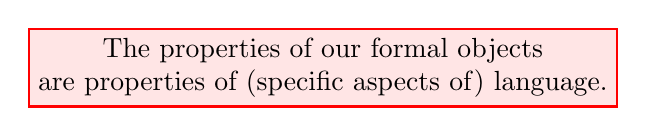
\begin{tikzpicture}
        \node[draw=red, fill=red!10, thick, align=center]
            {The properties of our formal objects\\ are properties of (specific aspects of) language.};
    \end{tikzpicture}
\end{center}
%
The theoretical task of proving formal properties of strictly local languages has suddenly morphed into an empirically minded investigation of phonology.

\section{Exploring Strictly Local Languages}

\subsection{A Proper Hierarchy of Strictly Local Languages}
The examples discussed so far suggest that the power of strictly local grammars increases with the size of the locality domain.
This is indeed the case, but is best proved by recourse to the strictly local languages.
If we order the strictly local languages by the size of their locality domain, we get a proper hierarchy: one level properly subsumes the next.
Denoting the class of strictly $k$-local languages by $\SL_k$, we have $\SL_k \subsetneq \SL_{k-1}$ for all $k \geq 0$.

This is a complex claim, as it asserts that each strictly $k$-local language is strictly $k+1$-local, but that the opposite does not hold for some languages.
Following our standard strategy, we establish lemmata for these weaker claims and then combine them into the original theorem.
%
\begin{lemma}
    It holds for every $k \geq 0$ that if language $L$ is strictly $k$-local, then $L$ is also $k+1$-local.
\end{lemma}
%
The proof for this lemma is slightly more complicated than anything we have seen so far, but behind the notation lies a very simple idea:
the size of the locality domain can be increased from $k$ to $k+1$ by padding the edge markers and by combining two overlapping $k$-grams into a single $k+1$-gram.
Consequently, for every strictly $k$-local grammar there is an equivalent strictly $k+1$-local one.
%
\begin{proof}
    If $L$ is strictly $k$-local then it is generated by some positive strictly $k$-local grammar $G$ over some alphabet $\Sigma$.
    Let $G'$ be the smallest set such that for all $k$-grams $g_1, g_2 \in G$
    %
    \begin{itemize*}
        \item if $g_1$ starts with $\LeftEdge$, then $\LeftEdge g_1 \in G'$,
        \item if $g_1$ ends with $\RightEdge$, then $g_1 \RightEdge \in G'$,
        \item if $g_1 \is a_1 a_2 \cdots a_{k}$ and $g_2 \is a_2 \cdots a_k a_{k+1}$, then $a_1 a_2 \cdots a_k a_{k+1} \in G'$.
    \end{itemize*}
    %
    Clearly $G'$ is finite and can therefore be interpreted as a positive $k+1$-local grammar.
    We show that $L = L(G')$, thus establishing that $L$ is $k+1$-local.
    
    If $w \in L(G')$, then $\Bigrams[k+1](w)$ is a subset of $G'$.
    All $k+1$-grams with multiple edge markers have a corresponding $k$-gram with one edge marker less, which is contained in $G$.
    All other $k+1$-grams are split into two $k$-grams by removing the first or the last symbol.
    Each $k$-gram is once again contained in $G$, so $\Bigrams[k](w) \subseteq G$ and hence $w \in L(G) = L$.
    Since $w$ was arbitrary we have $L(G') \subseteq L$.

    If $w \in L$, then $\Bigrams[k](w)$ is a subset of $G$.
    Assume towards a contradiction that $\Bigrams[k+1](w)$ is not a subset of $G'$.
    Then $w$ contains some $k+1$-gram $g_3$ that is not a member of $G$.
    If $g_3$ starts or ends with two edge markers, then the corresponding $k$-gram with only one of the two markers cannot have been part of $G$, contradicting our initial assumption.
    In all other cases, $g_3$ is built from two overlapping $k$-grams $g_1$ and $g_2$, at least one of which is not contained in $G$.
    But then $\Bigrams[k](w)$ is not a subset of $G$, contradicting once more our initial assumption.
    It follows, then, that $\Bigrams[k+1](w)$ is a subset of $G'$ after all, wherefore $L \subseteq L(G')$.
\end{proof}
%
\begin{examplebox}[Converting Bigrams Into Trigrams]
    Consider the strictly $2$-local language $(\String{ab})^+$ and its positive strictly $2$-local grammar $G$ with the bigrams $\LeftEdge a$, $\String{ab}$, $\String{ba}$, and $b\RightEdge$.
    In order to construct an equivalent strictly $3$-local grammar, we have to pad out the edge markers and combine overlapping bigrams.
    So $\LeftEdge a$ and $b \RightEdge$ become $\LeftEdge\LeftEdge a$ and $\RightEdge\RightEdge b$, respectively.
    We also see that $\LeftEdge a$ overlaps with $\String{ab}$, so we can combine them into $\String{\LeftEdge a b}$.
    The same procedure produces $\String{ab \RightEdge}$ from $\String{ab}$ and $b \RightEdge$.
    Finally, $\String{ab}$ and $\String{ba}$ overlap in two ways depending on which one is put in front of the other, so that we obtain two trigrams from them: $\String{aba}$ and $\String{bab}$.
    This exhausts the number of possible combinations. 
    The strictly $3$-local grammar is shown below:
    %
    \begin{center}
        \begin{tabular}{lll}
            \String{\LeftEdge\LeftEdge a}
            &
            \String{aba}
            &
            \String{b \RightEdge\RightEdge}
            \\
            \String{\LeftEdge a b}
            &
            \String{bab}
            &
            \String{a b \RightEdge} 
        \end{tabular}
    \end{center}
    %
    This grammar generates all strings of $(\String{ab})^+$, and only those.
\end{examplebox}

\begin{lemma}
    For every $k$ there is some strictly $k+1$-local language that is not strictly $k$-local.
    \label{lem:SLMath_SL-HierarchyProper}
\end{lemma}
%
\begin{proof}
\Note{%
    This proof uses a finite language, but the lemma holds even if we only consider infinite languages.
    Try to generalize the proof along these lines.
}
    Consider the finite language $L$ that contains only the string $a^k$, i.e.\ the string with $k$ consecutive $a$s.
    It is generated by the strictly $k+1$-local grammar $\setof{\LeftEdge a^k, a^k \RightEdge}$.
    However, $\Bigrams[k](a^k) = \setof{\LeftEdge a^{k-1}, a^k, a^{k-1} \RightEdge} = \Bigrams[k](a^n)$ for every $n \geq k$, so a strictly $k$-local grammar that generates $a^k$ also generates all these $a^n$ and thus a proper superset of $L$.
\end{proof}
%
\begin{theorem}
    For all $k \geq 0$, $\SL_k \subsetneq \SL_{k+1}$.    
\end{theorem}

Now we know for sure that the size of the locality domain has a direct effect on generative capacity.
This is hardly surprising, but still far from trivial --- in Chapter~\ref{cha:REG} we will encounter a very similar formalism for which all $k \geq 2$ have exactly the same power.


\subsection{Relation to Finite Languages}

Remember that the list phonology model of Lecture~\ref{cha:ListPhonology} was restricted to lists of finite length, so it could only generate finite languages.
This restriction is empirically inadequate as it conflicts with the assumption that the list of phonological words in a given natural language is infinite and fails to handle nonce words and linguistic creativity in general.
But not only is the list phonology model restricted to finite languages, it adds insult to injury with its ability to generate all finite languages.
Every finite language is a viable natural language phonology according to the list model, and we have already seen why this is typologically untenable.
The class of finite languages is the class that is least likely to provide an insightful or empirically adequate model of language, so we should strive to work with formalisms that cannot generate this class.

The strictly local languages are a marked improvement over the list phonology model in this respect, but only if one adopts the right perspective.
First, it is obvious that strictly local languages can be infinite, so not every strictly local language is finite.
Let us make this claim fully explicit via a proof.
We already know that every strictly $k$-local language is strictly $k+1$-local, so all we need is an example of a language that is both infinite and strictly $1$-local language.

\Note{%
Further reflection reveals that almost every $1$-local language is infinite.
In fact, there are only two $1$-local languages that are finite.
Can you define them?
\emph{Hint}: One of them is strictly $0$-local.
}
%
\begin{lemma}
    There is a strictly $1$-local language that is infinite.
\end{lemma}
%
\begin{proof}
    Let $\posG{G} \is \setof{\LeftEdge, a, \RightEdge}$.
    Then $L(\posG{G}) = \setof{\emptystring, a, \String{aa}, \String{aaa}, \ldots} = a^*$, which is infinite.
\end{proof}
%
\begin{corollary}
    For every $k \geq 1$, $\SL_k$ contains an infinite language.
\end{corollary}
%
This is a welcome result because it shows that no matter what size of locality domain we pick, we are never restricted to just finite languages.
An even more appealing property of strictly local languages is that for every level of the infinite hierarchy there are some finite languages that cannot be defined.
Consequently, strictly local grammars improve on the list phonology model in that they cannot define just about any arbitrary phonological systems.
%
\begin{theorem}
    For every $k \geq 1$, there is some finite language that is not contained in $\SL_k$. 
\end{theorem}
%
\begin{proof}
    Pick an infinite language that is generated by some strictly $k$-local grammar $G$ over alphabet $\Sigma$.
    Discard from $G$ all $k$-grams that start with $\LeftEdge$ or end in $\RightEdge$.
    The resulting set is a finite language $L$.
    We show that $L$ is not strictly $k$-local.

    Since $G$ generates an infinite set, it must contain (not necessarily distinct) $k$-grams $a \stringcat u$ and $u \stringcat b$, where $a,b \in \Sigma$ and $u \in \Sigma^{k-1}$.
    Note that both $a \stringcat u$ and $u \stringcat b$ belong to $L$, whereas $a \stringcat u \stringcat b$ does not.
    But $\Bigrams[k](a \stringcat u) \cup \Bigrams[k](u \stringcat b) = \Bigrams[k](a \stringcat u \stringcat b)$, and consequently every strictly $k$-local grammar that generates $a \stringcat u$ and $u \stringcat b$ also generates $a \stringcat u \stringcat b$.
    Hence $L$ is not strictly $k$-local.
\end{proof}
%
The proof above is rather sneaky.
It exploits the fact that every strictly $k$-local grammar is a finite set of strings of length $k$, but this very set can also be viewed as a finite language.
This is an interesting perspective: a strictly $k$-local grammar $G$ is a finite language $L_G$ coupled with a specific algorithm $A$ for creating a new language from $L_G$.
If we try to generate $L_G$ via a second strictly $k$-local grammar, this grammar automatically uses the algorithm $A$, so for certain choices of $L_G$ the grammar generates additional strings via $A$ that do not belong to $L_G$.

Viewing grammars as languages will seem odd to many linguists, who think of the grammar as the knowledge the speaker has acquired about their language, whereas the language is the output produced from this knowledge.
But that is an ontological distinction.
It is a useful distinction to make when outlining the research program of linguistics, its goals, problems, and promises.
It highlights that modern linguistics is about human cognition rather than merely describing individual languages as abstract systems of structures and rules that exist independent of the speaker's cognitive ability to use them.
The latter view dates back to Structuralism, and there are good reasons why it was abandoned.
As useful as the ontological mandate may be, though, it has no say over what mathematical tricks we may avail ourselves of.
Equating grammars with languages can be useful in some cases.
Here it furnishes a proof about the limits of strictly local languages, and in Ch.~\ref{cha:Derivations} it will open up completely new methods of constructing syntactic grammars.

If you still find all of this horribly confusing, do not despair:
there is a much simpler proof that does not blur the distinction between grammars and languages and instead uses the same trick that we already encountered in the proof of Lem.~\ref{lem:SLMath_SL-HierarchyProper}.
%
\begin{proof}
    Consider the finite language that consists only of the string $a^k$.
    Note that $\Bigrams[k](a^k) = \setof{\LeftEdge a^{k-1}, a^k, a^{k-1} \RightEdge} = \Bigrams[k](a^{k+1})$.
    Thus every strictly $k$-local grammar that generates $a^k$ also generates $a^{k+1}$.
    This entails that no strictly $k$-local grammar generates the finite language $\setof{a^k}$.
\end{proof}
%
Why would anyone ever want to use the more complicated proof if there is a much simpler one?
In poetic terms: because the journey is the destination.
Proofs aren't just about establishing results, they tell us why a specific result holds and hence provide us with deeper insights.
The simpler proof does not highlight that each strictly local grammar it itself a finite language, an obvious yet nonetheless surprising fact.
New perspective like this are always useful.
Remember the Keenan-Moss credo:
%
\begin{center}
    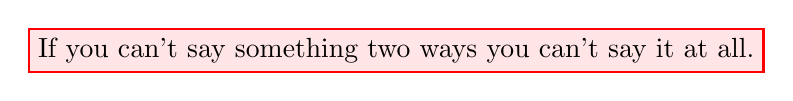
\begin{tikzpicture}
        \node[draw=red, fill=red!10, thick]
            {If you can't say something two ways you can't say it at all.};
    \end{tikzpicture}
\end{center}
%
This isn't restricted to definitions, it also extends to proofs.
The more routes take us towards a specific result, the better.

One important point that both proofs share is that they presuppose that the size of the locality domain is fixed to some $k$.
Hence they do not apply if we consider the whole class of strictly local languages, which turns out to properly subsume the class of finite languages.
%
\begin{theorem}
    Every finite language is strictly local.
\end{theorem}
%
\begin{proof}
    Suppose that $L$ is a finite language, the longest string of which has length $k - 1$, $k \geq 1$.
    We define a $k$-local grammar $G$ that consists of the $k$-grams $\LeftEdge^i \stringcat w \stringcat \RightEdge^j$, where $w \in L$, $w$ has length $l < k$, and $i + j + l = k$.
    Since every $k$-gram starts with $\LeftEdge$ or ends in $\RightEdge$, $L(G) = L$, wherefore $L$ is strictly $k$-local.
\end{proof}
%
We see that the relation between strictly local languages and finite languages is more involved than one would expect.
Without restrictions on the size of the locality domain, the strictly local languages include all finite languages.
However, the class of strictly $k$-local languages and the class of finite languages are incomparable --- they have a non-empty intersection, but neither subsumes the other (cf.\ Fig.~\ref{fig:SLMath_SL-Fin}).
So assuming that $k$ is fixed for natural language phonology, e.g.\ as part of Universal Grammar, strictly local grammars are a good approximation of local processes in phonology.
They can handle infinity and do not incorrectly predict languages to vary freely across all dimensions.
In particular, they naturally give rise to iterated local processes such as progressive vowel harmony.
%
\begin{figure}[htpb]
    \centering
    \begin{tikzpicture}[
    lang/.style = {rounded corners, thick, fill, fill opacity=.5}
    ]
    \node (sl0) at (0,0) {$\SL_0$};
    \node (sl1) at (4em,0) {$\SL_1$};
    \node (sln) at (10em,0) {$\SL_n$};
    \node (sl) at (16em,0) {$\SL$};
    
    \node (fin) at (-6em,0) {$\FIN$};

    \node (dots1) at ($(sl1) !.5! (sln)$) {\ $\cdots$};
    \node (dots1) at ($(sln) !.5! (sl)$) {\ $\cdots$};

    % rectangles for language classes
    \begin{pgfonlayer}{background}
        % SL 
        \draw[lang,blue!45] ($(fin.north west)+(-1.5em,2.5em)$) rectangle ($(sl.south east)+(1.5em,-2.5em)$);

        % SL_n
        \draw[lang,blue!15] ($(sl0.north west)+(-2em,1.25em)$) rectangle ($(sln.south east)+(.5em,-1.25em)$);

        % SL_1
        \draw[lang,blue!10] ($(sl0.north west)+(-1em,.5em)$) rectangle ($(sl1.south east)+(.5em,-.5em)$);
        
        % SL_0
        \draw[lang,blue!5] ($(sl0.north west)+(-.5em,.25em)$) rectangle ($(sl0.south east)+(.5em,-.25em)$);

        % Fin
        \draw[lang,red!35] ($(fin.north west)+(-1em,2em)$) rectangle ($(fin.south east)+(4em,-2em)$);
    \end{pgfonlayer}
\end{tikzpicture}

    \caption{Relation between strictly local and finite languages}
    \label{fig:SLMath_SL-Fin}
\end{figure}

\subsection{Substring Substitution Closure}
\label{sub:SLMath_SubstitutionClosure}

In several of the preceding proofs we have used the fact that a strictly local grammar sometimes ``overshoots the target''.
A finite language $L$ may not be in $\SL_k$ because a strictly $k$-local grammar that tries to generate $L$ will also end up generating other strings outside of $L$.
But a strictly $k+1$-local grammar may be able to do a point landing and generate all and only those strings that are members of $L$.
What this shows is that a strictly $k$-local grammar only has perfect precision within its locality domain of size $k$, beyond that it has to generalize.
This generalization step is what allows strictly local grammars to generate infinite languages, making it the true source of their power.

Crucially, though, strictly local grammars don't just generalize randomly, quite to the contrary: all strictly local grammars generalize in the same fashion, irrespective of the size of their locality domain.
Their generalization strategy is already implicit in the definition of strictly local languages, which categorizes strings as well-formed or ill-formed according to their set of $k$-grams.
If two strings have exactly the same set of $k$-grams, then either both are well-formed or both are ill-formed.

But it is quite hard to tell what this condition implies for the overall shape of the string languages.
Given a string language $L$, how can we tell whether $L$ is strictly local?
Fortunately strictly local languages are uniquely characterized by a property called \emph{substring substitution closure}.
%
\begin{definition}[Local Substring Substitution Closure]
    A language $L$ satisfies \emph{$k$-local substring substitution closure} iff there is some $k \geq 1$ such that if $L$ contains both $u \stringcat x \stringcat v$ and $u' \stringcat x \stringcat v'$, where $x$ has length $k - 1$, then $L$ also contains $u \stringcat x \stringcat v'$.
\end{definition}
%
\begin{theorem}
    A language is in $\SL_k$ iff it satisfies $k$-substring substitution closure.
\end{theorem}
%
Let us look at a couple of examples first before wading through the proof of the theorem.

\begin{examplebox}[A Substring Substitution Closed Language]
    We have already seen that the language $(\String{ab})^+$ is strictly $2$-local as it is generated by the grammar $\setof{\LeftEdge a, \ngram{ab}, \ngram{ba}, b \RightEdge}$.
    Now we can also verify this via substring substitution closure.
    For instance, we can line up $\String{abab}$ and $\String{abababab}$ to show that the language must also contain $\String{ababab}$.
    %
    \[
        \begin{array}{rcll}
                          & x &              & \\
            \String{ab}   & a & \String{b}   & \in L\\
            \String{abab} & a & \String{bab} & \in L\\\hline
            \String{ab}   & a & \String{bab} & \in L
        \end{array}
    \]
    %
    Notice how $x$ is a single symbol since its length must be $k-1 = 2 - 1 = 1$.
    Also, we could have established the membership of $\String{ababab}$ more succinctly using just $\String{abab}$ or $\String{abababab}$.
    \[
        \begin{array}{rcll}
                        & x &              & \\
            \String{ab} & a & \String{b}   & \in L\\
                        & a & \String{bab} & \in L\\\hline
            \String{ab} & a & \String{bab} & \in L
        \end{array}
        %
        \qquad
        %
        \begin{array}{rcll}
                          & x &                & \\
            \String{ab}   & a & \String{babab} & \in L\\
            \String{abab} & a & \String{bab}   & \in L\\\hline
            \String{ab}   & a & \String{bab}   & \in L
        \end{array}
    \]
\end{examplebox}
%
Since substring substitution closure fails if even a single string is missing from the set, it is usually not a good way of showing that a language is strictly local --- if the language in question is infinite, one cannot show via specific substitutions that it is suffix substitution closed.
However, suffix substitution closure is an excellent way of showing that a language is \textbf{not} strictly local by giving a single example of a missing string.
%
\begin{examplebox}[A Language that Fails Subtree Substitution Closure]
    Consider the language $(\String{aa})^+$, the variant of $(\String{ab})^+$ where all $b$s have been replaced by $a$s.
    This language is not strictly local as it fails $k$-local substring substitution closure for any choice of $k$.
    Suppose $k$ is an even number:
    %
    \[
        \begin{array}{rcll}
            & x & & \\
        a & a \cdots a & a & \in L \\
          & a \cdots a &   & \in L \\\hline
        a & a \cdots a &   & \notin L\\
        \end{array}
    \]
    %
    A minimally different pattern is used if $k$ is odd.
    No matter what the value of $k$, the language is not suffix substitution closed and thus not strictly local.
    You might find this surprising given that the only difference to $(\String{ab})^+$ is the replacement of $b$ by $a$.
    This highlights another property of strictly local languages: the alphabet plays a crucial role in what languages are definable.
\end{examplebox}
%
\begin{proof}
    We now show that a language $L$ is strictly $k$-local iff it is closed under $k$-local substring substitution.
    
    \paragraph{Left to right}
    Note first that substring substitution closure is trivially satisfied if $L$ contains no strings of length strictly greater than $k-1$, for then all strings take the form $\emptystring \stringcat x \stringcat \emptystring$ with respect to $k$-local substring substitution.
    Suppose, then, that $s_1$ and $s_2$ are strings of $L$ with length strictly greater than $k-1$ such that $s \is u_1 \stringcat x \stringcat v_1$ and $s_2 \is u_2 \stringcat x \stringcat v_2$.
    If $s_1 = s_2$, then $u_1 \stringcat x \stringcat v_2 = s_1 = s_2$, so substring substitution closure is not violated.
    If $s_1 \neq s_2$, then it must be the case that $\Bigrams[k](u_1 \stringcat x \stringcat v_2) \subseteq \Bigrams[k](s_1) \cup \Bigrams[k](s_2) \subseteq G$, where $G$ is a strictly $k$-local grammar with $L(G) = L$.
    It follows immediately that $s_1 \stringcat x \stringcat v_2$ is a member of $L(G)$ and thus a member of $L$. 
    This exhausts all possible cases, showing that $L$ is indeed closed under $k$-local substring substitution.

    \paragraph{Right to left}
    Suppose $L$ is closed under $k$-local substring substitution, and let $G \is \bigcup_{w \in L} \Bigrams[k](w)$ be a positive strictly $k$-local grammar.
    It suffices to establish $L(G) = L$, which entails that $L$ is strictly $k$-local.

    It is easy to see from the definition of $G$ that $L \subseteq L(G)$.
    Showing that $L(G) \subseteq L$ requires a fairly lengthy proof that is omitted here.
    The curious reader is referred to \citet[19--21]{Rogers07}.
\end{proof}

\subsection{Closure Properties}

Suffix substitution closure is --- as its name implies --- a \emph{closure property}.
One says that an object $o$ is closed under an operation iff applying this operation to elements of $o$ yields only elements of $o$.
In other words, the operation never takes us outside of $o$.
The natural numbers, for instance, are closed under addition since the sum of two natural numbers is yet again a natural numbers.
But they are not closed under subtraction because, say, $2-5$ yields $-3$, which is an integer but not a natural number.
Suffix substitution closure simply means that a language is closed under the operation of substituting suffixes in a specific way.

But of course there are many other operations that can be applied to a language, and it will be interesting to see whether strictly local languages are closed under them.
In particular the basic set-theoretic operations of intersection, union, and relative complement are of interest since they tell us how we can build strictly local languages from smaller ones.

Let us look at closure under intersection first.
This one is particularly important because of the close correspondence that negative strictly local grammars establish between constraints on the one hand and languages on the other.
If every $k$-gram corresponds to a well-formedness constraints, then one would expect that one can get the intersection of two languages by simply conjoining their respective well-formedness constraints.
That is indeed the case.
%
\begin{lemma}
    The class of strictly $k$-local languages is closed under intersection, $k \geq 0$.
\end{lemma}
%
\begin{proof}
    We prove that for any two strictly local languages generated by (positive) grammars $G_1$ and $G_2$, $L(G_1) \cap L(G_2) = L(G_1 \cap G_2)$.
\Note{Give an analogous proof using negative grammars.}
    We first show $L(G_1) \cap L(G_2) \subseteq L(G_1 \cap G_2)$.
    Let $w$ be an arbitrary string belonging to both $L(G_1)$ and $L(G_2)$, i.e.\ $w \in L(G_1) \cap L(G_2)$.
    Then every $k$-gram of $w$ is contained in both $G_1$ and $G_2$, so $w \in L(G_1 \cap G_2)$.
    Since $w$ is arbitrary, we have $L(G_1) \cap L(G_2) \subseteq L(G_1 \cap G_2)$.
    The same reasoning can be applied in the other direction, yielding $L(G_1 \cap G_2) \subseteq L(G_1) \cap L(G_2)$.
    These two facts jointly imply $L(G_1) \cap L(G_2) = L(G_1 \cap G_2)$.
\end{proof}
%
% fixme: hw: spell out the second subset relation
%
Closure under intersection, too, can be used to prove that a language is not strictly local.
Suppose we know that $L$ is strictly local, but we have a hard time showing that $L'$ is not strictly local.
Then we can instead try to show that $L \cap L'$ is not strictly local, as this immediately implies the non-locality of $L'$, too.
%
% fixme: example!

One might expect that closure under union holds too since one can simply take the union of the grammars, but this does not work as expected.
The union of two grammars $G_1$ and $G_2$ often generates a superset of the union of $L(G_1)$ and $L(G_2)$.
Do not even try to look for a smarter strategy to build a grammar for the union of two strictly local languages, there is none that works in all cases.
%
\begin{lemma}
    The class of strictly $k$-local languages is not closed under union. 
\end{lemma}
%
\begin{proof}
    We give an example of two strictly $2$-local languages whose union is not strictly $2$-local.
    The proof can easily be adapted for arbitrary values of $k$.

    Let $L_1 \is \setof{\mathit{ab}}$ and $L_2 \is \setof{\mathit{b}, \mathit{bb}, \mathit{bbb}, \ldots}$.
    \Note{``w.l.o.g.''\ is short for ``without loss of generality'' and is meant to indicate that the proof can easily be adapted to cases that are not covered by the assumption.}
    Assume w.l.o.g.\ that all strictly $2$-local grammars are positive.
    Then any strictly $2$-local grammar that generates $L_1$ must contain the bigrams $\LeftEdge a$, $\mathit{ab}$, and $b \RightEdge$.
    Similarly, a strictly $2$-local grammar generating $L_2$ must contain the bigrams $\LeftEdge b$, $\mathit{bb}$, and $b \RightEdge$.
    Therefore a strictly $2$-local grammar that generates all strings in $L_1 \cup L_2$ must contain at least these bigrams.
    But such a grammar also generates the string $\mathit{abb}$, which is not part of $L_1 \cup L_2$.
    Hence there is no strictly $2$-local grammar that generates all the strings in $L_1 \cup L_2$ and nothing else, so $L_1 \cup L_2$ is not a strictly $2$-local language.
\end{proof}
%
The proof above only shows that the union of two strictly $k$-local languages is not guaranteed to be strictly $k$-local.
However, it will still be strictly $k+1$-local.
So it is still conceivable that the whole class of strictly local languages is closed under union, that is to say, the union of two strictly $k$-local languages may still be strictly $m$-local for some $m > k$.
But this is not always the case, either.
Intuitively, union can give rise to long-distance dependencies that cannot be enforced with strictly local grammars.
%
\begin{lemma}
    The class of strictly local languages is not closed under union.
\end{lemma}
%
\begin{proof}
    Consider the two strictly $2$-local languages $L \is \String{ab^+}$ and $L' \is \String{b^+ a}$.
    Their union is not closed under $k$-local substring substitution closure for any $k \in \NatNum$ since $a b^k a \notin L \cup L'$, so it is not strictly local.
\end{proof}

Abstract as it may be, this result is of immediate importance for our investigation of phonology.
If the union of two arbitrary strictly local languages were also strictly local, then we would expect that phonological processes can always apply disjunctively.
Consider the following example: some languages have sibilant harmony, while others have vowel harmony.
Each process can be equated with the set of strings that satisfy the respective harmony pattern.
If we take the union of these two sets, we get the set of strings that satisfy sibilant harmony or vowel harmony.
If that set were intersected with some natural language's phonology --- which is an abstract way of saying that we force the constraint represented by that set onto the language --- then words in that language are well-formed as long as they obey sibiliant harmony or vowel harmony, but they need not obey both.
This is extremely unnatural. If a language has two phonological processes, then words must usually obey both.
It is not the case that satisfying one constraint grants you \emph{carte blanche} to ignore the other.
The closure properties of strictly local languages can explain this fact: intersection (= constraint conjunction) always yields a potential natural language phonology, union (=constraint disjunction) may not.
The assumption that local phonological processes fit within the bounds of strictly local languages thus makes a typological prediction: if two constraints apply in a disjunctive fashion as indicated above, then these two constraints must be such that their union is also strictly local --- which rules out a great number of strictly local languages.
%
%fixme: hw: extend proof to case where both languages are infinite
%fixme: hw: extend proof to arbitrary k

The previous two lemmata also imply that closure under relative complement does not hold.
%
\begin{lemma}
    The class of strictly local languages is not closed under (relative) complement.
\end{lemma}
%
\begin{proof}
    By De Morgan's law $L_1 \cup L_2 = \complementof{\complementof{L_1} \cap \complementof{L_2}}$.
    If the class of strictly local languages were closed under both complement and intersection, it would thus be closed under union, too.
    Since closure under intersection holds while closure under union does not, closure under relative complement cannot hold, either.
\end{proof}
%
%fixme: hw: give a proof by example
You may find this result surprising because the complement of a strictly local grammar is a strictly local grammar.
But in general $\complementof{L(G)}$ differs from $L(\complementof{G})$, just like $L(G_1) \cup L(G_2)$ is not guaranteed to be $L(G_1 \cup G_2)$.
These differences illustrate why it is so important to distinguish between grammars and the languages they generate.

Another property not enjoyed by strictly local languages is closure under concatenation.
Given two languages $L_1$ and $L_2$, their concatenation contains all strings that can be obtained by concatenating a string of $L_1$ with a string of $L_2$.
In mathematical jargon: $L_1 \stringcat L_2 \is \setof{ u \stringcat v \mid u \in L_1, v \in L_2}$.
%
\begin{lemma}
    The class of strictly local languages is not closed under concatenation.
\end{lemma}
%
\begin{proof}
    Consider the strictly $2$-local languages $L_1 \is \String{(a^+ c)^+}$ and $L_2 \is \String{(a^+ d)^+}$.
    Their concatenation is not closed under $k$-local substring substitution closure:
    \[
        \begin{array}{rcll}
            \String{a^{k-1}cad} & a^{k-1} & \String{d}    & \in L_1 \stringcat L_2\\
                          & a^{k-1} & \String{cada^{k-1}d} & \in L_1 \stringcat L_2\\\hline
            \String{a^{k-1}cad} & a^{k-1} & \String{cada^{k-1}d} & \notin L_1 \stringcat L_2
        \end{array}
    \]
\end{proof}
%
Closure under string concatenation is yet another unnatural closure property since it implies that the rules of a grammar can switch completely at some point in the string.
The fact that English and French are natural languages would make the ludicrous prediction that a system where the first part of the word follows the rules of English phonology and the second part the French rules is a possible natural language phonology.
Lack of closure under string concatenation thus is a very robust universal of the class of natural languages and one that we do not want in our formalism, either.

We finish with yet another missing closure property.
A relabeling of a language is a function that replaces each symbol in all strings by some other symbol.
More precisely, let $\Sigma$ and $\Omega$ be two alphabets and $r: \Sigma \rightarrow \Omega$ be a total function (that is to say, it produces some output for every symbol of $\Sigma$).
Then for every string $w = w_1 w_2 \cdots w_n$, we let $r(w) \is r(w_1) r(w_2) \cdots r(w_n)$ and $r(L) \is \setof{ r(w) \mid w \in L}$.
%
\begin{lemma}
    The class of strictly local languages is not closed under relabelings.
\end{lemma}
%
\begin{proof}
    We have already seen that $(ab)^+$ is strictly 2-local whereas the relabeling $(aa)^+$ is not strictly $k$-local for any $k \in \NatNum$.
    But the former is the image of the latter under a relabeling that replaces all $b$s by $a$s.
\end{proof}
%
This is a very important result as it ties directly into the abstractness debate in generative phonology.
Suppose that we are allowed to have all kinds of hidden structure in our phonological representation, e.g.\ a basic syllable template or feet.
Then we could assume that the language $(aa)^+$ is underlyingly equipped with a CV-template, so that we should rather think of it as $(a_C a_V)^+$.
This language is strictly local (it is a notational variant of $(ab)^+$), so $(aa)^+$ is strictly local under a mapping that removes unpronounced structure.
In Chapter~\ref{cha:REG} we will see that this is a very dangerous route to take: hidden structure pushes strictly local languages to a level of power where all phonological processes are equally simple.
This eradicates all distinctions between processes and takes us back to the undesirable egalitarianism of the list phonology model.

A summary of all the (non-)closure properties is given in Tab.~\ref{tab:SLMath_ClosureProperties}.
Notice that the closure properties of strictly local languages is closely in line with what we see natural languages, whereas the finite languages get almost everything wrong.
%
\begin{table}
\centering
    \begin{tabular}{rcccl}
        \toprule
        \textbf{Closure under\ldots} & \textbf{FIN} & \textbf{SL} & \textbf{Natural} & \textbf{Typological Issue}\\
        \midrule
        Intersection & \yes & \yes & \yes (?) & all constraints can apply conjunctively\\
        Union & \yes & \no & \no & all constraints can apply disjunctively\\
        Complement & \yes & \no & \no & constraint opposites are possible constraints\\
        Concatenation & \yes & \no & \no & distinct constraints for word halves\\
        Relabeling & \yes & \no & \no (?) & abstractness debate\\
        \bottomrule
    \end{tabular}
\caption{Comparison of closure properties and their linguistic relevance}
\label{tab:SLMath_ClosureProperties}
\end{table}

\section{Implications for Phonology}
Our mathematical expedition has taught us a surprising amount about phonology.
First of all, all local phonological dependencies (including those spanning across word boundaries) can be handled by strictly local grammars, a very simple formalism with few cognitive requirements.
The model comes with a minimal memory burden as it only requires the speaker to keep track of a small number of $k$-factors.
It is also very fast: recognition via a scanner takes linear time and can be carried out in an incremental online fashion.
Lookup of $k$-factors in the grammar takes at most logarithmic time using binary search, and even faster search methods can be implemented.
With a hash table or prefix tree, lookup is practically instantaneous.

But strictly local grammars also capture essential properties of phonological competence.
They are analytic in nature and thus capable of generating infinite languages, which solves the problems the list phonology model had with linguistic creativity and nonce words.
The special relation between strictly $k$-local languages and finite languages also means that certain typological pitfalls are avoided.
Not every random collection of strings is predicted to be a valid phonological system, and grammars generating an infinite language generalize in a linguistically plausible fashion by determining the well-formedness of strings as a composite function of the local domains.

We have also seen that strictly local languages lack closure properties that do not hold of natural languages either.
The union or relative complement of a natural language's phonotactics is not guaranteed to be a valid phonological system for a natural language, just like the class of strictly local languages is not closed under these operations.
The increase of power brought about by relabelings also cautions us against using hidden structures and highly abstracted alphabets, an issue that has been discussed at length in phonology and that will occupy us at various points for the rest of the course.

%fixme: non-closure under composition
%       contrast with closure properties of FIN

%fixme:
%hw: complete proof of positive-negative equivalence
%hw: implement k to k+1 converter
